\section{Coinductive Data Types}
\label{sec:coinductive-types}
\newcommand{\bisim}{\text{\texttildelow}}
% Thomas
%#########
% Hvad er en coinduktiv type? (eliminationsregler) (typeteori)
% Hvorfor coinduktive typer / hvad kan de bruges til?
% Simple eksempler
% Uortodokse eksempler (fx partiality)
% Lazy evaluation (i.e. Haskell-style) vs. distinction between coinductive and
%% inductive data

% Ny viden: Coinduktive typer
%#########
Inductive types have widespread applications across the field of computer
science in general, and functional programming in particular. Because they are
defined in terms of a finite and disjoint set of constructors, which determine
the internal structure of any element of such type, an induction
principle can be formulated for any inductive type. The implications are that
properties about functions on inductive types can be proven by structural
induction. Indeed, by the Curry-Howard
isomorphism\,\citep{Curry1934,Howard80,Wadler2014}, functions on inductive types
can be \emph{implemented} as proofs by structural induction. By nature, only
finite objects can be constructed from inductive types, since they have an
internal tree structure. As such, a leaf must be reached at some
point. Concretely, an inductively defined standard list structure must be ended
with the empty list in order to be well-defined.

Coinductive types are dual to inductive types. Intuitively, they can be defined
in terms of a finite and disjoint set of \emph{destructors}, which as a whole
determine the observable behaviour of elements of such type. Infinite objects
can be constructed from coinductive types, because they can have an internal
graph structure. This allows for the definition of circular structures, which
makes them suitable for reasoning about values that may unfold indefinitely,
e.g. processes\,\citep{Sangiorgi2011}. Coinductive types are often defined in
terms of abstract mathematics and category theory, and a formal definition of
coinductive types has been given by Jacobs and
Rutten\,\citep{Jacobs97atutorial}. We will not proceed with the formal
definition here, but instead provide a more intuitive explanation.

To define a coinductive type, which we may call $B$, means to define its observable behaviour: At any
given time, what can we observe about an element of $B$? If for any given $B$,
we wish to observe $n$ different things, we can define $B$ by $n$ destructors,
as shown in Figure~\ref{fig:coinductive_type_n_destructors}. 
\begin{figure}[H]
  \centering
  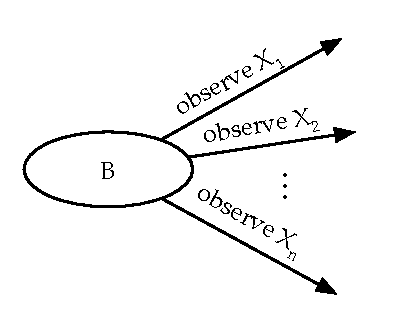
\includegraphics{figures/general_coind_intuition_prod_coinductive}
  \caption{An illustration of a coinductive type with $n$ destructors defining
    its observable behaviour.}
\label{fig:coinductive_type_n_destructors}
\end{figure}
In Idris, a
definition of $B$ may be given as follows, where T$_1$,T$_2$,$\cdots$,T$_n$ are
Idris types, either inductive or coinductive:
\begin{lstlisting}[mathescape]
corecord B where
  X$_1$ : T$_1$
  X$_2$ : T$_2$
    $\vdots$
  X$_n$ : T$_n$
\end{lstlisting}
However, this definition implies that all of these observations can be made for
any element of $B$. If we wish to define observations that can only be made on
\emph{some} elements of a coinductive type, the observable behaviour must
reflect 

% An inductive type is defined in terms of the ways it can be constructed. In the
% simple case where an inductive type $B$ has only one constructor, this may be
% illustrated as in Figure~\ref{fig:inductive_type_one_constructor}. In
% particular, we can construct $B$ by giving ${X_1,\,X_2,\,\cdots,\,X_n}$ as
% arguments to its sole constructor. To define the same $B$ coinductively, we must
% define it in terms of its observable behaviour (i.e. its destructors). What may
% we expect to observe about $B$? 



\begin{figure}[h]
  \centering
  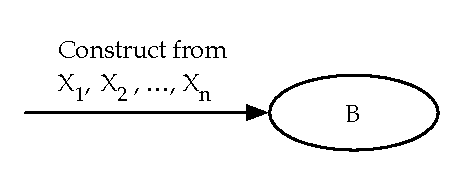
\includegraphics{figures/general_coind_intuition_prod_inductive}
  
  \caption{An illustration of an inductive type with one constructor which has
    $n$ input parameters.}
\label{fig:inductive_type_one_constructor}
\end{figure}


% Before making matters more concrete, we
% proceed with a formal definition.

% \begin{definition}[\textit{Coinductive data type}]
% \label{def:coinductive_data_type}
%   Given an endofunctor $F$, a coinductive data type is an element of a final
%   coalgebra ($X$, $c$), where $X$ is the carrier and $c$ is a \emph{structure
%     map} $X\,\to\,F(X)$\,\citep{Jacobs97atutorial,Kozen2012}.
% \end{definition}

% While we will not claim to fully understand the category theory underlying
% Definition~\ref{def:coinductive_data_type}, we do have a working intuition of
% its implications. For instance, the endofunctor ${F(X)=A\times X}$ together with
% the final coalgebra ($X$, $(head, tail) : X\to A\times X$) characterizes the set
% of infinite streams, and can be implemented as a coinductive data type in Idris
% as follows:

% \begin{lstlisting}[mathescape]
% codata Stream : Type $\to$ Type where
%   (::) : (head : a) $\to$ (tail : Stream a) $\to$ Stream a
% \end{lstlisting}

% In this example, we define the observable behaviour of \texttt{Stream} as a
% whole to be the conjunction of the behaviour defined by the destructors \texttt{head} and \texttt{tail}. As a consequence, we can informally state
% that the constructor \texttt{(::)} models the structure map. This intuition extends to infinitely branching trees over an endofunctor
% ${F(X)=A\times X\times X}$ and a coalgebra ($X$, ${(value,lefttree,righttree) : X\to
% A\times X\times X)}$, possibly infinite lists over an endofunctor ${F(X)=1 + A\times X}$ and a coalgebra ($X$, ${(unfold) : X\to
% 1 + A\times X)}$, and so on. Note that when the endofunctor has a top-level sum structure,
% as for possibly infinite lists, the structure map is not split into separate
% destructors, since further analysis of the observed behaviour is needed.


\subsection{Coinduction}
% Definition by elimination
% Coinduction principle
Just as inductive types give rise to induction principles, coinductive types
give rise to coinduction principles. We will not provide a formal definition of
coinduction here, but instead give an example of coinductive reasoning. For the
interested reader, a formal definition is given by Kozen and
Silva\,\citep{Kozen2012}. Dual to induction, the Curry-Howard isomorphism
enables us to implement functions on coinductive data by coinduction. In
Figure~\ref{fig:proof_by_coinduction}, we give a simple example of a proof by
coinduction in Idris. Specifically, we show that the infinite stream of
\texttt{ones} is \emph{bisimilar} (\bisim) to the result of mapping the successor
constructor (\texttt{S}) over the infinite stream of zeros. Informally, a bisimulation is a relation between state transition
systems which denotes when two such systems have the same external behaviour. A
formal definition is given by Sangiorgi\,\citep[Section~1.4]{Sangiorgi2011}.
\begin{figure}[h]
\begin{lstlisting}[mathescape]
%default total

corecord Stream : Type $\to$ Type where
   head : Stream a $\to$  a
   tail : Stream a $\to$ Stream a
     
corecord BisimStream : (a : Type) $\to$ Stream a $\to$ Stream a $\to$ Type where
   phead : BisimStream a s t $\to$ head s = head t
   ptail : BisimStream a s t $\to$ BisimStream a (tail s) (tail t)

map : (a $\to$ b) $\to$ Stream a $\to$ Stream b
&head map f s = f (head s)
&tail map f s = map f (tail s)

zeros : Stream Nat
&head zeros = Z
&tail zeros = zeros

ones : Stream Nat
&head ones = S Z
&tail ones = ones

eq : BisimStream Nat ones (map S zeros)
&phead eq = Refl
&ptail eq = eq
\end{lstlisting}
  \caption{An example of a proof by coinduction in Idris. The clauses beginning
    with ``\&'' use our copatterns.}
\label{fig:proof_by_coinduction}
\end{figure}
The proof, given by the definition of \texttt{eq} in
Figure~\ref{fig:proof_by_coinduction}, proceeds as follows: 
\begin{framed}
\textbf{Theorem}: \texttt{ones} \bisim{} \texttt{map S zeros}. \\\\
\emph{Proof.} The proof proceeds by coinduction on the observed behaviour of \texttt{map~S~zeros}. The definitions used are the
ones given in Figure~\ref{fig:proof_by_coinduction}. First, we prove the case
for \texttt{head}, \texttt{head ones = head~(map~S~zeros)}:
\begin{align*}
   \texttt{head ones} &= \texttt{head (map S zeros)} \\
   \texttt{S Z} &= \texttt{S (head zeros)} \\
   \texttt{S Z} &= \texttt{S Z}
\end{align*}
Next, we show the case for \texttt{tail}, \texttt{tail ones} \bisim{} \texttt{tail
  (map S zeros)}:
\begin{align*}
   \texttt{tail (ones)}\, &\bisim\, \texttt{tail (map S zeros)} \\
   \texttt{ones}\,&\bisim\, \texttt{map\, S\, (tail\, zeros)} \\
   \texttt{ones} \,&\bisim\, \texttt{map S zeros} \qed
\end{align*}
The last step follows immediately from the coinduction hypothesis, i.e. {\texttt{ones}~\bisim{}~\texttt{map~S~zeros}}
\end{framed}
% ones ~ mapStream S zeros

% hd ones = hd (map S zeros)
% hd ones = S (hd zeros)
% S Z = S Z qed

% tl (ones) ~ tl (mapStream S zeros)
% tl (ones) ~ mapStream S (tl zeros)
% ones ~ mapStream S zeros BY COINDUCTION HYPOTHESIS!

By examining the implementation of \texttt{eq}, the reasoning may at first seem
oddly circular: the \texttt{tail} case is proven by an appeal to \texttt{eq}
itself. But since \texttt{eq} is productive, it can essentially provide us with
an infinite stream of proofs by reflexivity (\texttt{Refl}), and therefore holds
for an any unfolding of \texttt{ones} and \texttt{map S zeros}. In
our experience, a proof by coinduction often proceeds by identifying a productive
way of continually generating proofs.

\subsection{Coinductive Types by Lazy Evaluation}
% Coinductive types as inductive types (Jacobs)
Coinductive types can be encoded as lazily evaluated inductive types. This is
the approach followed in Idris (see Section~\ref{sec:coind-data-types}),
ensuring that infinite recursion never arises from an attempt to build an
infinite object by strict evaluation. 

% Theoretically, such an encoding is
% unproblematic, since any final coalgebra can be as an
% algebra\,\citep{JacobsCoalgebra}.

In languages where all data constructors are lazily evaluated, such as the
non-strict part of Haskell, coinductive types are almost provided ``for
free''. Indeed, Haskell makes no distinction between inductive and coinductive
types, which may leave us to question whether the distinction matters at
all. However, avoiding the distinction in general has at least two important
consequences. First, we may lose subject reduction in a dependently typed
system, since we cannot selectively disallow pattern matching on coinductive
types (we elaborate upon this issue in
Section~\ref{sec:recov-subj-reduct}). Secondly, we become unable to prove that
our language has the Church-Rosser property\,\citep{CR:36}, seeing as lazily
evaluating an infinitely recursive program may lead to a normal form when
strictly evaluating the same program may not. For Idris, the second problem is
the most dire, inasmuch as the total part of Idris is believed to have the
Church-Rosser property\,\citep{BradyIdrisImpl13}.

%Church-Rosser
%We cannot disallow pattern matching on coinductive data

% Start: Algebraiske data typer
% Hvad er en algebra (algebraic structure)?
% Hvad er en F-algebra?
% F-coalgebra
% Induktive og coinduktive typer
% eksempel
% Category theory nonsense?

% Algebraic data types are ubiquitous in functional programming, providing a
% concise way of defining data types.

% \begin{figure} 
% \begin{lstlisting}
% data Lam = Var String
%          | Abs String Lam
%          | App Lam Lam
% \end{lstlisting}
% \caption{The untyped lambda calculus defined as an algebraic data structure in a
% Haskell-like language. For simplicity, strings are used for identifiers.}
% \end{figure}

%%% Local Variables:
%%% mode: latex
%%% TeX-master: "../../copatterns-thesis"
%%% End:
